\documentclass[a4paper, 12pt]{article}
\usepackage[utf8]{inputenc}
\renewcommand\familydefault{\sfdefault}
\usepackage[T1]{fontenc}
\usepackage[francais]{babel}
\usepackage[left=2.5cm,top=2.5cm,right=2.5cm,bottom=2.5cm]{geometry}
\usepackage{graphicx}
\usepackage{minted}
\usemintedstyle{colorful}
\usepackage{float}
\floatplacement{figure}{H}
\usepackage{authblk}
\usepackage{enumitem}
\usepackage{hyperref} 
\hypersetup{
	colorlinks,
	citecolor=black,
	filecolor=black,
	linkcolor=black,
	urlcolor=blue
}

\usepackage{mdframed}

\begin{document}

\title{Petits comptes entre amis} 
\author{Steven Liatti} 
\affil{\small Développement et services web - Prof. Stéphane Malandain} 
\affil{\small Hepia ITI 3\up{ème} année} 
\maketitle

\begin{figure}
	\begin{center}
		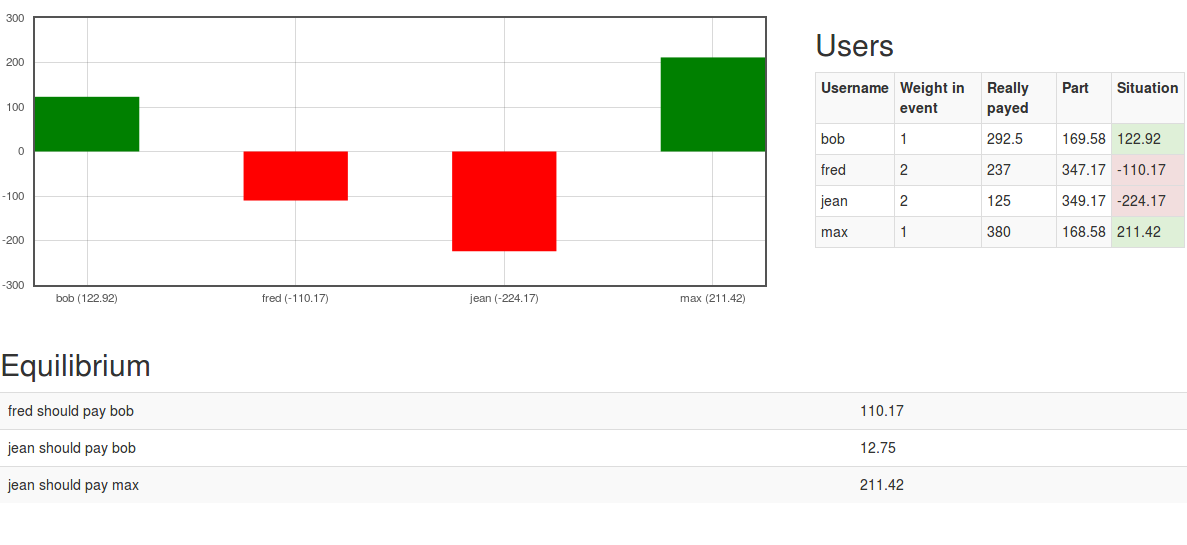
\includegraphics[width=1.0\textwidth]{intro.png}
	\end{center}
\end{figure}
\newpage

\tableofcontents 
\listoffigures

\newpage

\section{Introduction}
\subsection{Description}
Le but de ce mini-projet est de réaliser un site en php permettant à des amis de noter et
partager les dépenses effectuées par et pour le groupe au cours de vacances
communes. Lorsque l’une des personnes fait des courses, par exemple, elle l’enregistre.
Chacun enregistre les dépenses qui concernent le groupe. Ainsi, à la fin du séjour (ou à
tout moment) on peut savoir qui a payé quoi et surtout ce que chacun doit aux autres
personnes du groupe d’amis.

\subsection{Technologies utilisées}
\begin{itemize}
	\item Base de données :
	\begin{itemize}
		\item \href{https://www.mysql.com/}{MySQL}, avec
		\item \href{https://www.mysql.com/products/workbench/}{MySQL Workbench} (pour la création du schéma)
	\end{itemize}
	\item Back-end :
	\begin{itemize}
		\item \href{https://httpd.apache.org/}{Apache}, serveur HTTP
		\item \href{http://php.net/}{PHP}, avec
		\item \href{https://silex.symfony.com/}{Silex}, micro framework PHP basé entre autres sur \href{https://symfony.com/}{Symfony}, déployé avec \href{https://getcomposer.org/}{Composer}
		\item \href{https://twig.symfony.com/}{Twig}, moteur de templates pour PHP (utilisé de concert avec Silex)
	\end{itemize}
	\item Front-end :
	\begin{itemize}
		\item \href{http://getbootstrap.com/}{Bootstrap} pour le design en CSS
		\item \href{https://jquery.org/}{jQuery}
		\item \href{http://www.flotcharts.org/}{Flot}, un plugin pour dessiner des graphiques avec jQuery
	\end{itemize}
\end{itemize}


\section{Base de données}
Les technologies imposées pour la base de données de ce travail pratique sont SQLite ou MySQL. J'ai choisi d'utiliser 
MySQL, car je suis familier avec. J'ai profité de cette occasion pour découvrir et utiliser Workbench, un programme 
permettant de modéliser les tables et relations d'une base de données de manière graphique. Une fois le model terminé, 
Workbench offre la possibilité de l'exporter en instructions SQL (création de tables et contraintes).
\bigbreak

Mon schéma est constitué des tables suivantes :
\begin{figure}
	\begin{center}
		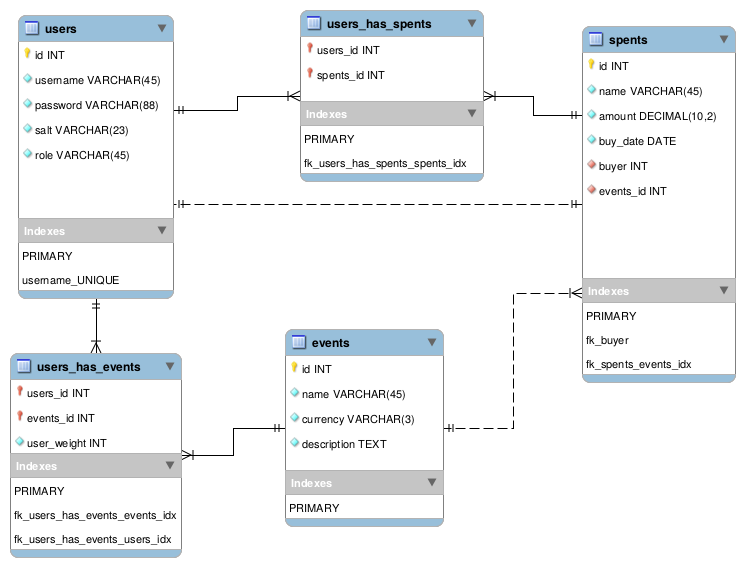
\includegraphics[width=1.0\textwidth]{database.png}
	\end{center}
	\caption{Schéma de la base de données relationnelle}
\end{figure}
Il y a 3 tables principales : les utilisateurs, les événements et les dépenses. 2 autres tables secondaires 
font la liaison entre les utilisateurs et les événements et les utilisateurs et les dépenses respectivement 
(liaison Many-To-Many). La table des utilisateurs possède un champ \mintinline{sql}{salt} et un autre 
\mintinline{sql}{role}, ils sont nécessaires au fonctionnement de Silex (explications plus loin). Le poids 
de chaque utilisateur au sein d'un événement est indiqué dans la table croisée 
\mintinline{sql}{users_has_events}. 
Chaque dépense référence l'acheteur (dans \mintinline{sql}{users}) et l'événement lié (dans \mintinline{sql}
{events}). Ce schéma représente l'interface minimum pour les données de ce travail, mais il a l'avantage 
d'être simple à comprendre et à maintenir.

\section{Back-end}
Je profite également de ce TP pour appréhender Silex, un micro framework PHP dérivé de Symfony (que j'ai eu 
l'occasion de tester), beaucoup plus léger que son grand frère mais tout de même robuste et modulaire. Il 
bénéficie d'un grand nombre de modules à ajouter, en vrac : système de templates, connexion à la base de données, 
routes, etc.

\newpage

\subsection{Architecture MVC avec Silex}
Grâce à Silex, mon architecture respecte le design pattern \href{https://en.wikipedia.org/wiki/Model-view-controller}{MVC}.
On peut configurer Silex pour que le code source, défini dans le répertoire \mintinline{text}{src}, soit ajouté 
au mécanisme de chargement automatique (autoloading) géré par Composer. Pour que cela fonctionne, il faut que le code 
source respecte le standard \href{http://www.php-fig.org/psr/psr-4/}{PSR-4}.
Voici l'arborescence du site :
\begin{mdframed}[linecolor=black, topline=true, bottomline=true, leftline=true, rightline=true]
	\inputminted[breaklines,breaksymbol=,linenos,stepnumber=5,tabsize=2]{php}{tree.txt}
	\label{tree}
\end{mdframed}
% \begin{figure}
% 	\begin{center}
% 		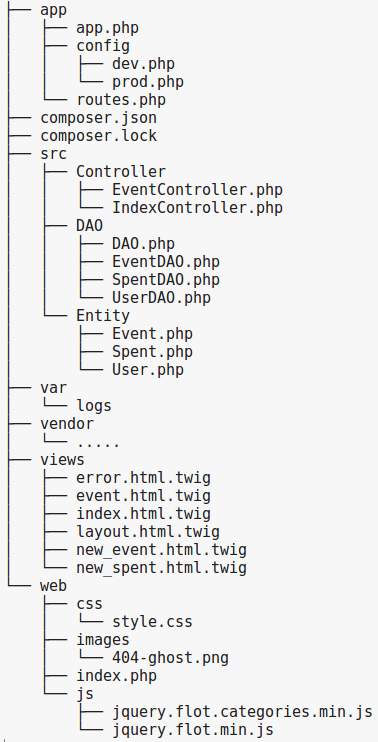
\includegraphics[width=0.5\textwidth]{tree.png}
% 	\end{center}
% 	\caption{Arborescence du site}
% \end{figure}

\begin{itemize}
	\item app : fichiers de config et routes
	\item composer.json : fichier de dépendances
	\item src : fichiers source PHP ("POPO", DAO, Contrôleurs)
	\item var : logs
	\item vendor : fichiers sources des composants Silex/Symfony
	\item views : fichiers de vues en Twig
	\item web : fichiers CSS, JS, images, etc. publics livrés au client
\end{itemize}

\subsection{Composants Silex}
Silex fournit plusieurs composants vraiment pratiques et très efficaces. Les composants suivants m'ont été 
particulièrement utiles :
\begin{itemize}
	\item Un composant de sécurité qui gère le login des utilisateurs
	\item Un composant de construction de formulaires
	\item Un composant pour se connecter à la base de données
	\item Un composant de rendu de templates (Twig)
	\item Un composant permettant de facilement appliquer des contraintes pour valider les données
\end{itemize}

\subsection{Routage et configuration}
Dans le dossier \mintinline{text}{app} se trouvent les fichiers de configuration (pour MySQL notamment) et les 
déclarations/configurations des modules et composants récupérés grâce à Composer (dans \mintinline{php}{app/app.php}).
Le point d'entrée du site est \mintinline{text}{web/index.php}. C'est le contrôleur frontal, c'est par ici que 
toutes les requêtes passent (grâce au fichier de configuration d'Apache \mintinline{text}{.htaccess}). 
Il instancie l'objet principal \mintinline{php}{$app} et fait suivre aux fichier de routes. Silex permet de 
définir des routes, c'est-à-dire des points d'entrée dans l'application. À chaque route est associée une action 
(requête GET et/ou POST) définie dans un contrôleur. Pour ce site, j'ai défini 6 routes : page d'accueil (avec 
formulaires de connexion et d'inscription), page d'un événement, nouvel événement, nouvel dépense, suppression 
d'événement et suppression de dépense.

\subsection{Contrôleurs}
Les contrôleurs sont le socle de ce site, c'est ici que sont récupérées les requêtes et les données (grâce aux 
DAO) et construits les formulaires et les vues. Une fonction \mintinline{php}{xxxAction()} d'un contrôleur a 
pratiquement toujours la forme suivante : test si la page est accessible par le client qui la demande, récupération 
des données (voir la sous-section \ref{data_model_access}), si besoin construction/vérification 
des formulaires et enfin rendu de la vue ou redirection vers une page donnée.

\subsubsection{\mintinline{php}{IndexController.php}}
Ce contrôleur gère les actions de la page principale. Si un utilisateur est connecté, il lui affiche les 
événements auxquels ils participe. Sinon, deux formulaires, de login et d'inscription, sont affichés. Grâce au 
composant de sécurité intégré, j'ai facilement pu mettre en place le login utilisateur. Il m'a suffit de 
configurer quelques réglages dans \mintinline{php}{app/app.php} : la route du formulaire de login et celle de la 
vérification du login (automatiquement faite), si les clients anonymes peuvent accéder à la page principale, 
la provenance des données utilisateurs, etc. : 
% (voir listing \ref{config_login}). 
% \begin{listing}[ht]
\begin{mdframed}[linecolor=black, topline=true, bottomline=true, leftline=true, rightline=true]
	\inputminted[breaklines,breaksymbol=,linenos,stepnumber=5,tabsize=2,firstline=26,lastline=39]{php}{../app/app.php}
	\label{config_login}
\end{mdframed}
	% \caption{Configuration du login utilisateur - \mintinline{php}{app/app.php}}
% \end{listing}

Si l'utilisateur s'inscrit, 
son formulaire est construit grâce au composant Silex, et lorsqu'il est reçu valide et conforme en retour, son 
mot de passe est hashé et le nouvel utilisateur est inscrit en base de données :
% (voir listing \ref{controller_register}).

% \begin{listing}[ht]
\begin{mdframed}[linecolor=black, topline=true, bottomline=true, leftline=true, rightline=true]
	\inputminted[breaklines,breaksymbol=,linenos,stepnumber=5,tabsize=2,firstline=22,lastline=56]{php}{../src/Controller/IndexController.php}
	\label{controller_register}
\end{mdframed}
	% \caption{Inscription d'un utilisateur - \mintinline{php}{src/Controller/IndexController.php}}
% \end{listing}

\subsubsection{\mintinline{php}{EventController.php}}
Ce contrôleur gère les actions des pages des événements et des dépenses. 

\subsection{Modèles, accès aux données}
\label{data_model_access}

\subsection{Vues}

\section{Front-end}
\subsection{CSS avec Bootstrap}
\subsection{jQuery et Flot JS}


\section{Conclusion}
\subsection{État actuel du projet}
Toutes les fonctionnalités demandées sont implémentées, pas de bugs connus.

\subsection{Propositions d'améliorations}
\begin{itemize}
	\item Tests unitaires
	\item Dans une situation réelle de production, on ne laisserait pas un utilisateur choisir parmi tous les autres 
			utilisateurs au moment de créer un nouvel événement. Il faudrait plutôt ajouter des adresses email, 
			d'utilisateurs déjà inscrits (ou non) sur le site, ainsi chaque invité peut rejoindre l'événement.
	\item Changer le code lié à la sélection du poids de l'utilisateur (lors d'un nouvel évenement) pour l'intégrer 
			avec le composant Form de Symfony.
\end{itemize}


\end{document}
